\documentclass{article}
\usepackage{graphicx} % Required for inserting images
\usepackage[left=1.5cm, right=2cm, top=2cm, bottom=2cm]{geometry}
\usepackage[T1]{fontenc}    %  (ą, ł, ś)
\usepackage[utf8]{inputenc} %  UTF-8
\usepackage[colorlinks=true, linkcolor=black,citecolor=black]{hyperref}
\usepackage[polish]{babel}
\usepackage[polish]{cleveref}
\usepackage{array}
\usepackage{float}
\usepackage{makecell}
\usepackage{multirow}
\usepackage{amsmath}
\usepackage{gensymb}
\usepackage[table]{xcolor}
\documentclass[12pt]{article}
\setlength{\intextsep}{5pt}   
\setlength{\floatsep}{3pt}     
\setlength{\textfloatsep}{5pt} 
\crefname{figure}{Rys.}{Rys.}
\Crefname{figure}{Rys.}{Rys.}
\crefname{section}{Rozd.}{Rozdziały}
\Crefname{section}{Rozd.}{Rozdziały}


\title{
\includegraphics[width=0.5\textwidth]{obrazy/logo-pwr-wm.png}\\[0.2cm] \Huge Sprawozdanie z Fizyki \\[0.2cm] \Huge Ćwiczenie 44a}
\author{\Large t0f1x }
\date{Wrocław, xx.xx.202x, Grupa nr. x }
\begin{document}
\maketitle
\tableofcontents
\newpage
\section{Wstęp}
\label{Wstep}
Ćwiczenie ma na celu zbadanie zależności oporu elektrycznego od temperatury dla dwóch różnych materiałów: metalu Próbka 1 oraz półprzewodnika Próbka 3 (dalej Próbka nr. 2).\\ Na podstawie wykonanych pomiarów wyznaczono temperaturowy współczynnik oporu metalu ($\alpha$) oraz szerokość przerwy energetycznej półprzewodnika ($E_g$).\\
Pomiary przeprowadzono z wykorzystaniem układu pomiarowego, w skład którego wchodziły: Miernik oporu M-3850, Jednostka sterująca zawierająca wyłącznik sieciowy, regulator temperatury, przełączniki 1, 2, 3, 4 podłączające wybraną próbkę do miernika oporu, grzejnik,  wentylator,wyłącznik wentylatora, Komora pomiarowa zawierająca badane próbki.
\newpage
\section{Wyniki}
    \begin{table}[h!]
    \centering
    \label{tab:pomiary_rezystancji}
    \resizebox{0.7\textwidth}{!}{
    \begin{tabular}{|c|c|c|c|c|}
    \hline
    \textbf{T [$\degree\text{C}$]} & \textbf{R1 [$\Omega$]} & \textbf{R2 [$\Omega$]} & \textbf{R3 [$\Omega$]} & \textbf{R4 [$\Omega$]} \\ \hline
    27  & 110.7 & 45.3 & 63.7 & 102.1 \\ \hline
    33  & 112.1 & 40.4 & 56.2 & 90.6  \\ \hline
    38  & 113.2 & 36.7 & 50.7 & 82.5  \\ \hline
    43  & 113.7 & 34.2 & 47.1 & 77.2  \\ \hline
    48  & 114.4 & 31.2 & 42.7 & 70.6  \\ \hline
    53  & 115.7 & 28.9 & 39.1 & 64.4  \\ \hline
    58  & 117.0 & 26.2 & 34.8 & 58.4  \\ \hline
    63  & 118.2 & 23.7 & 31.4 & 52.7  \\ \hline
    68  & 119.5 & 21.8 & 28.7 & 48.3  \\ \hline
    73  & 120.7 & 19.8 & 25.7 & 43.7  \\ \hline
    78  & 122.1 & 18.2 & 23.2 & 39.7  \\ \hline
    80  & 123.1 & 17.3 & 21.8 & 37.7  \\ \hline
    85  & 124.0 & 16.0 & 19.8 & 34.4  \\ \hline
    \end{tabular}
    }
    \caption{Wyniki pomiarów}
    \end{table}

Na podstawie pomiarów stwierdzamy, że próbka nr. 1 jest metalem, ponieważ jej opór rośnie wraz ze wzrostem temperatury, zaś pozostałe próbki są półprzewodnikami. 
\begin{figure}
    \centering
    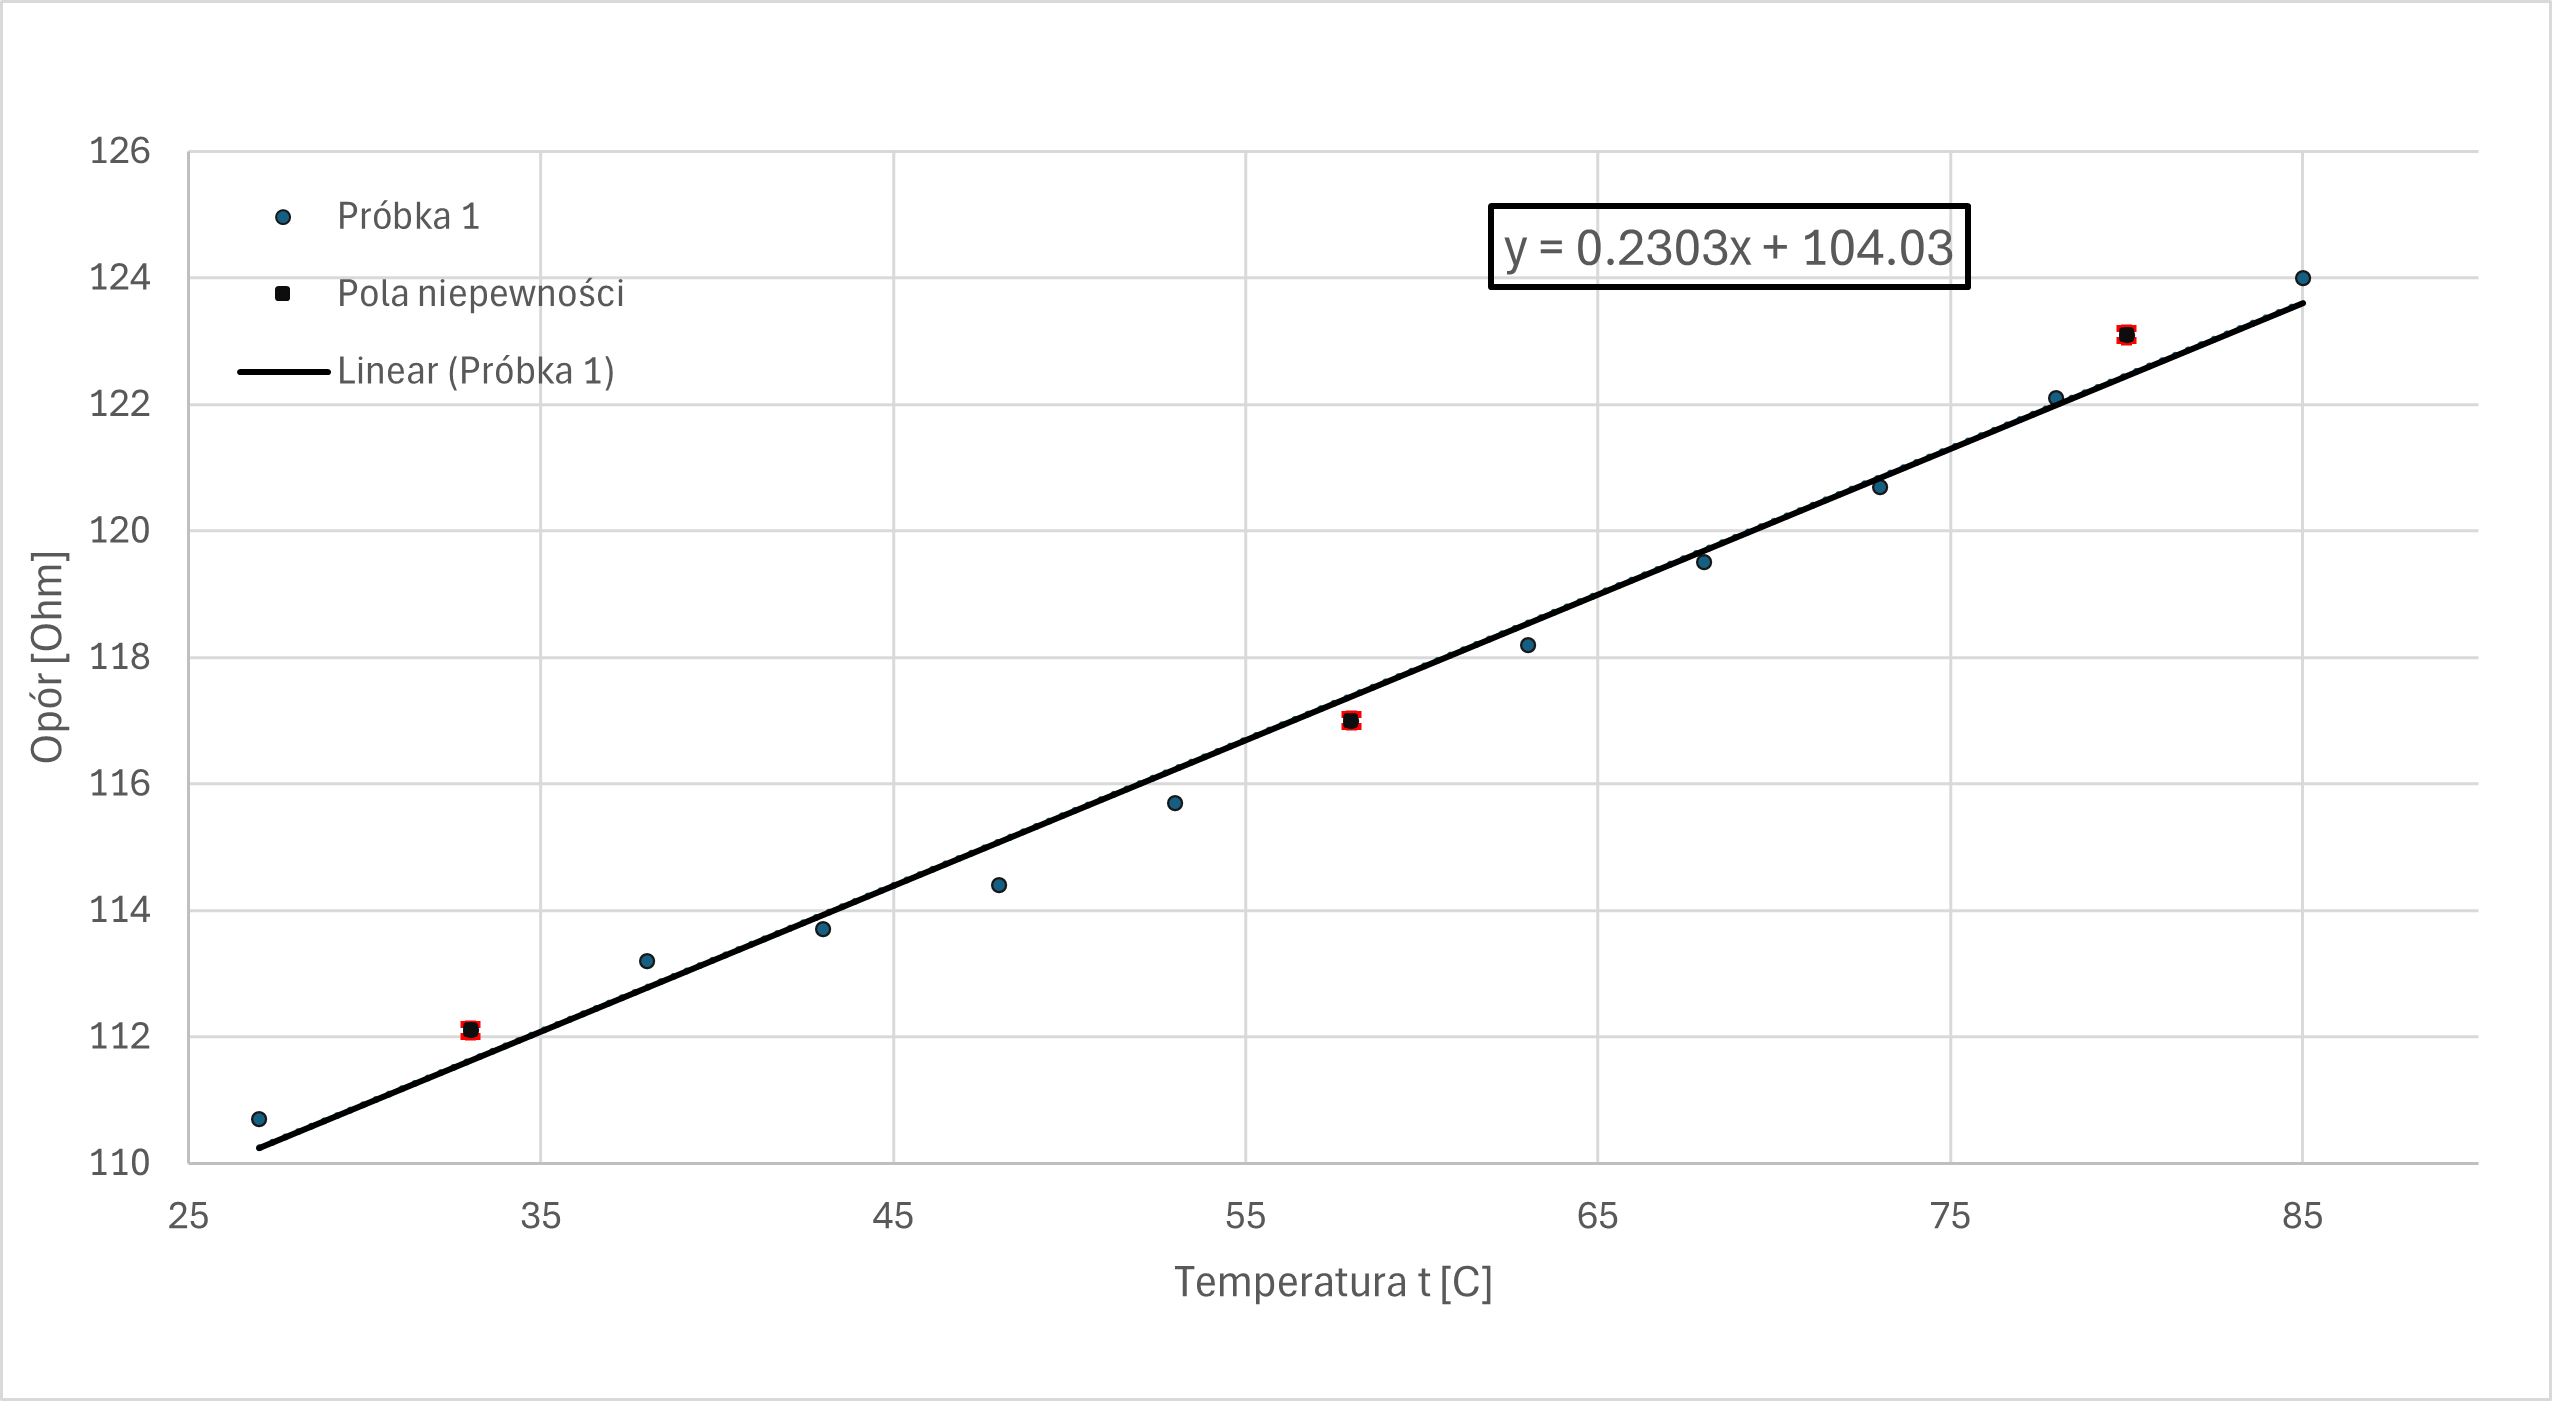
\includegraphics[angle=270,width=0.7\linewidth]{obrazy/Wykres1.png}
    \caption{Wykres 1}
    \label{fig:Wykres1}
\end{figure}
\begin{figure}
    \centering
    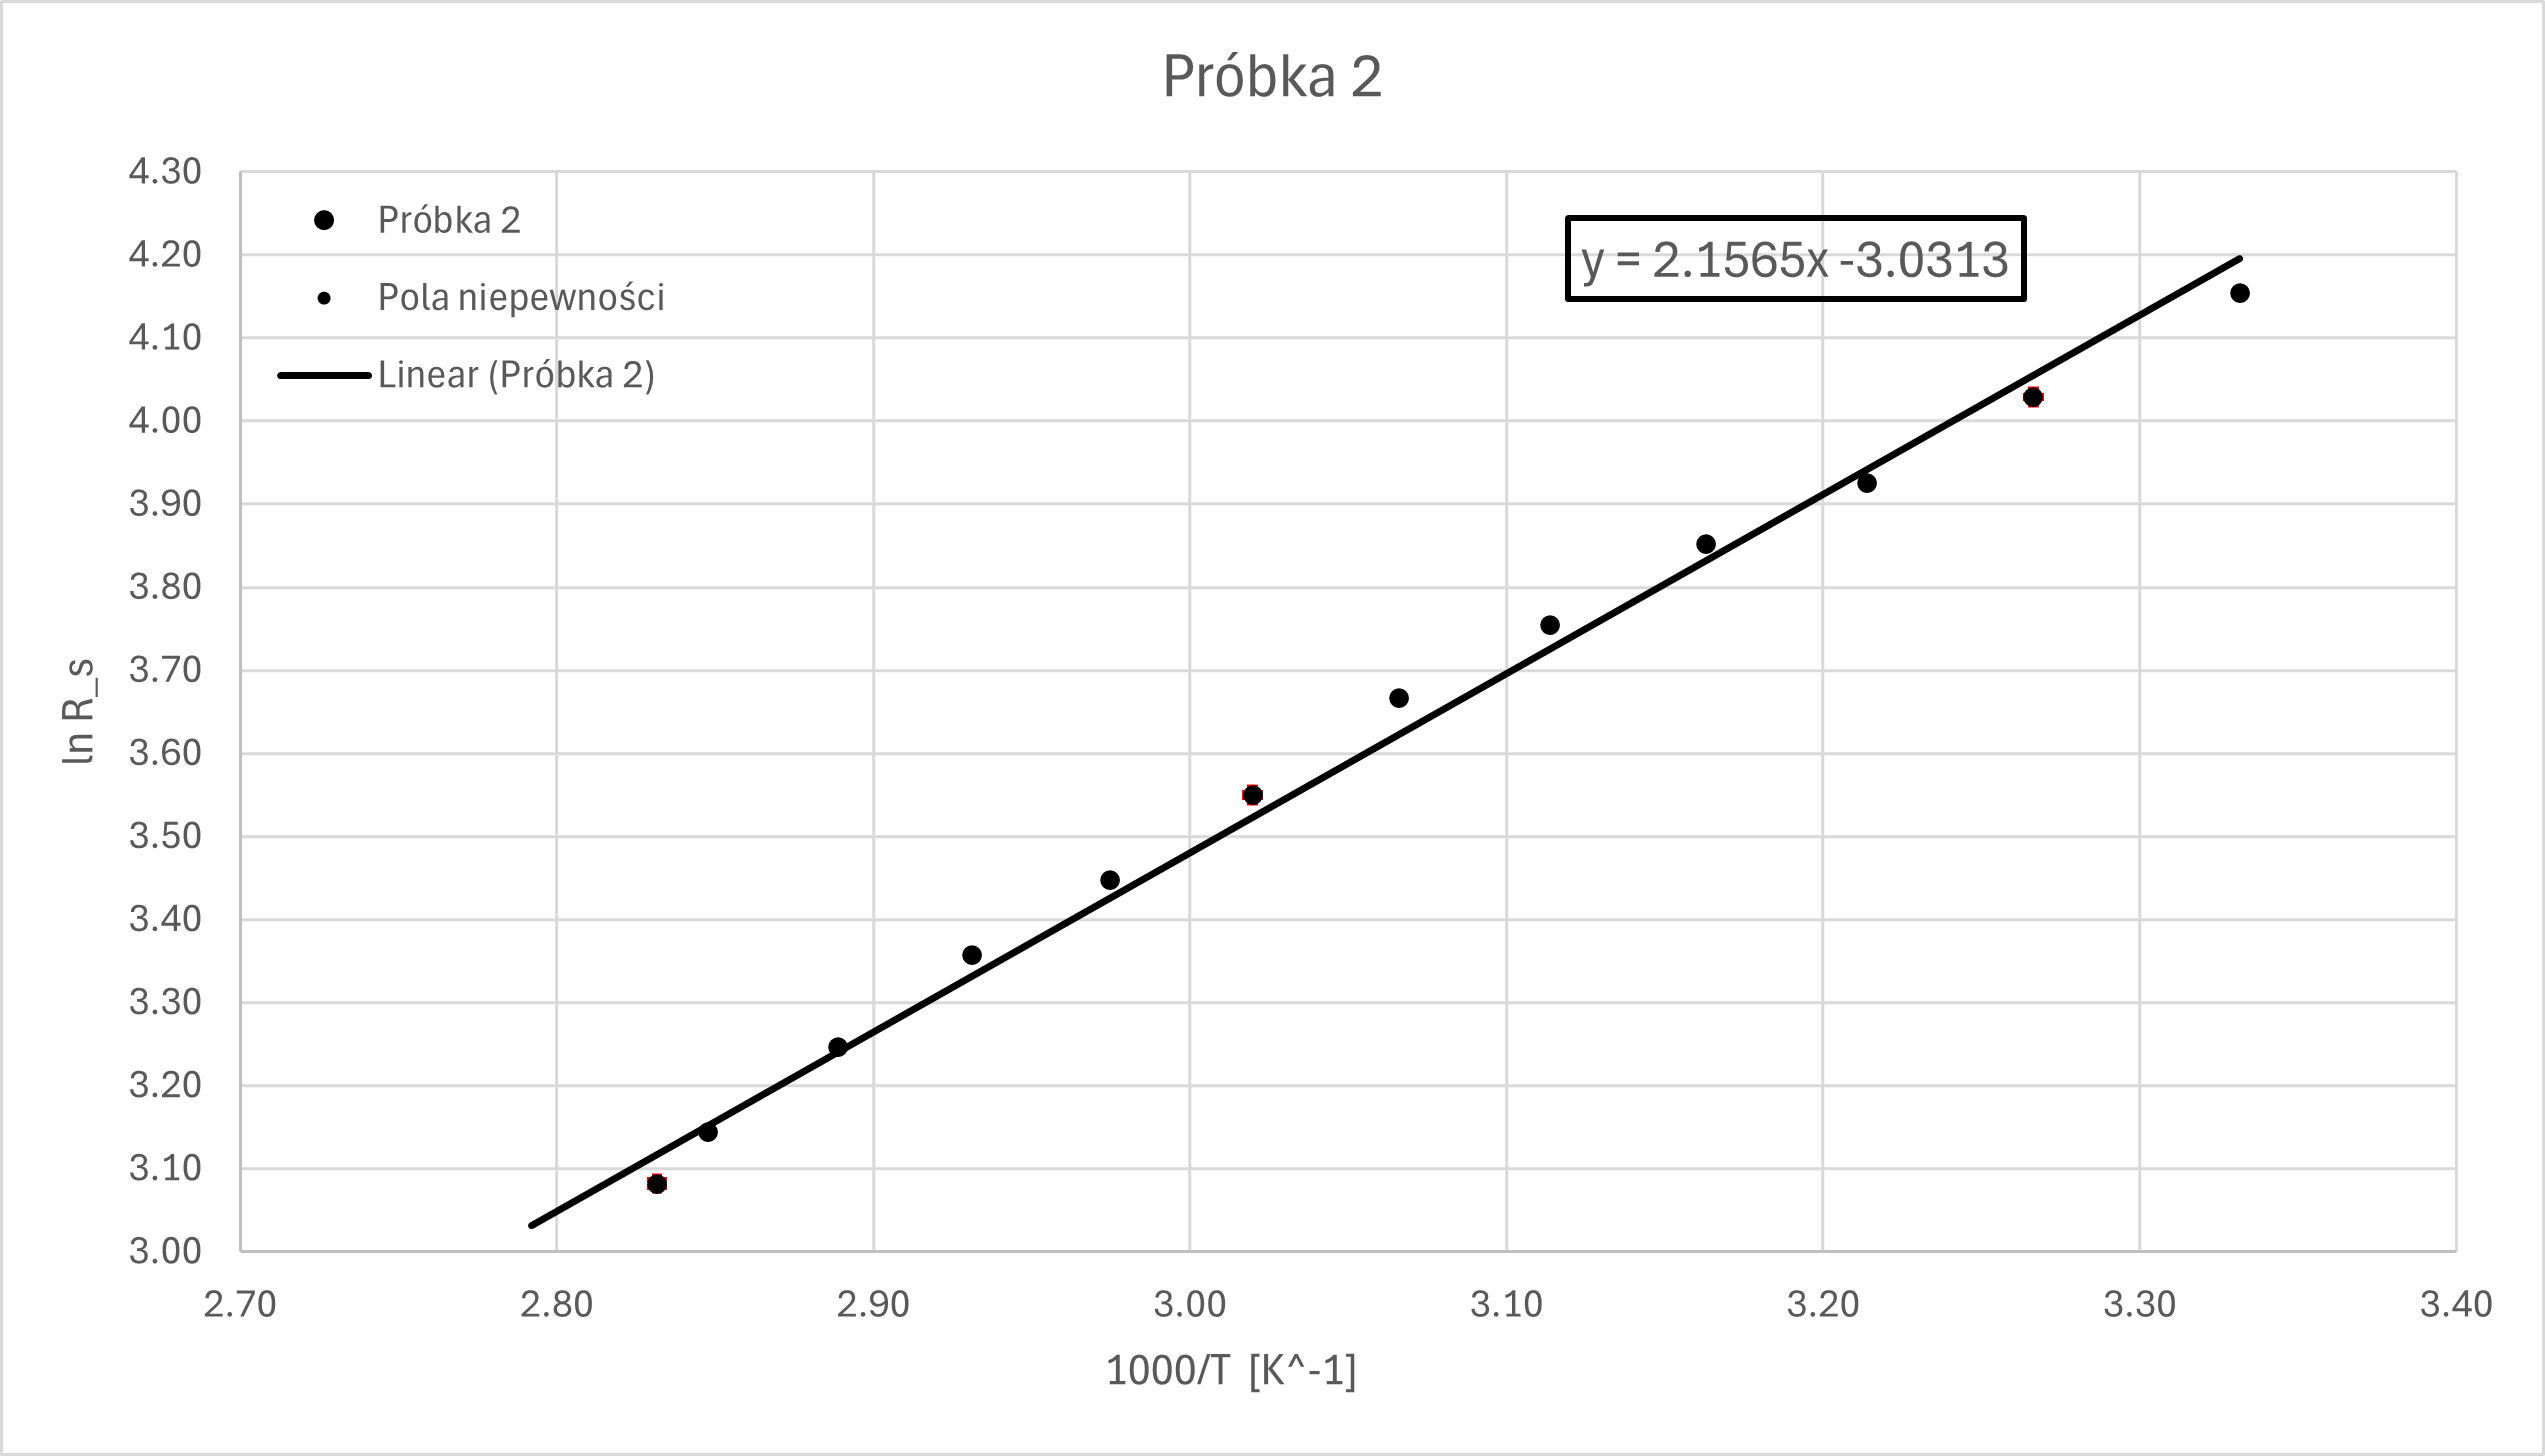
\includegraphics[angle=270,width=0.7\linewidth]{obrazy/Wykres2.png}
    \caption{Wykres 2}
    \label{fig:Wykres2}
\end{figure}

\newpage

\begin{table}[h]
    \centering
    \caption{Wyniki (Próbka 1)}
    \renewcommand{\arraystretch}{1.2}
    \resizebox{0.43\textwidth}{!}{
    \begin{tabular}{|c|c|c|c|c|c|}
    \hline
    \makecell{Lp.} & \makecell{$t$ \\ $[^{\circ}\text{C}]$} & \makecell{$R_m$ \\ $[\Omega]$} & \makecell{$a$ \\ $[\Omega/^{\circ}\text{C}]$} & \makecell{$b$ \\ $[\Omega]$} & \makecell{$\alpha$ \\ $[^{\circ}\text{C}^{-1}]$} \\    
    \hline
    1 & 27 & 110.7 & \multirow{13}{*}{0.2303} & \multirow{13}{*}{104.03} & \multirow{13}{*}{0.002214} \\
    \cline{1-3}
    2 & 33 & 112.1 & & & \\
    \cline{1-3}
    3 & 38 & 113.2 & & & \\
    \cline{1-3}
    4 & 43 & 113.7 & & & \\
    \cline{1-3}
    5 & 48 & 114.4 & & & \\
    \cline{1-3}
    6 & 53 & 115.7 & & & \\
    \cline{1-3}
    7 & 58 & 117.0 & & & \\
    \cline{1-3}
    8 & 63 & 118.2 & & & \\
    \cline{1-3}
    9 & 68 & 119.5 & & & \\
    \cline{1-3}
    10 & 73 & 120.7 & & & \\
    \cline{1-3}
    11 & 78 & 122.1 & & & \\
    \cline{1-3}
    12 & 80 & 123.1 & & & \\
    \cline{1-3}
    13 & 85 & 124.0 & & & \\
    \hline
    $\Delta X$ & 0.1 & 0.16 & \cellcolor{gray!30} & \cellcolor{gray!30} & \cellcolor{gray!30} \\
    \hline
    $u(X)$ & 0.058 & 0.092 & 0.0233 & 1.4035 & \cellcolor{gray!30} \\
    \hline
    $u_c(X)$ & \cellcolor{gray!30} & \cellcolor{gray!30} & \cellcolor{gray!30} & \cellcolor{gray!30} & 0.000226 \\
    \hline
    \end{tabular}
    }
    
    \label{tab:metal}
\end{table}

\begin{table}[h]
    \centering
    \renewcommand{\arraystretch}{1.2}
    \resizebox{0.65\textwidth}{!}{
    \begin{tabular}{|c|c|c|c|c|c|c|c|}
    \hline
    \makecell{Lp.} & \makecell{$t$ \\ $[^{\circ}\text{C}]$} & \makecell{$1000/T$ \\ $[\text{K}^{-1}]$} & \makecell{$R_s$ \\ $[\Omega]$} & \makecell{$\ln R_s$} & \makecell{$A$ \\ $[\text{K}]$} & \makecell{$E_g$ \ \cdot 10^{-20} \\ $[\text{J}]$} & \makecell{$E_g$ \\ $[\text{eV}]$} \\ 
    \hline
    1 & 27 & 3.3317 & 63.7 & 4.1542 & \multirow{13}{*}{2.1565} & \multirow{13}{*}{5.955} & \multirow{13}{*}{0.372} \\
    \cline{1-5}
    2 & 33 & 3.2664 & 56.2 & 4.0289 & & & \\
    \cline{1-5}
    3 & 38 & 3.2139 & 50.7 & 3.9259 & & & \\
    \cline{1-5}
    4 & 43 & 3.1631 & 47.1 & 3.8523 & & & \\
    \cline{1-5}
    5 & 48 & 3.1138 & 42.7 & 3.7542 & & & \\
    \cline{1-5}
    6 & 53 & 3.0661 & 39.1 & 3.6661 & & & \\
    \cline{1-5}
    7 & 58 & 3.0198 & 34.8 & 3.5496 & & & \\
    \cline{1-5}
    8 & 63 & 2.9749 & 31.4 & 3.4468 & & & \\
    \cline{1-5}
    9 & 68 & 2.9313 & 28.7 & 3.3569 & & & \\
    \cline{1-5}
    10 & 73 & 2.8890 & 25.7 & 3.2465 & & & \\
    \cline{1-5}
    11 & 78 & 2.8478 & 23.2 & 3.1442 & & & \\
    \cline{1-5}
    12 & 80 & 2.8317 & 21.8 & 3.0819 & & & \\
    \cline{1-5}
    13 & 85 & 2.7921 & 19.8 & 2.9857 & & & \\
    \hline
    $\Delta X$ & 0.1 & \cellcolor{gray!30} & 0.16 & \cellcolor{gray!30} & \cellcolor{gray!30} & \cellcolor{gray!30} & \cellcolor{gray!30} \\
    \hline
    $u(X)$ & 0.058 & \cellcolor{gray!30} & 0.092 & \cellcolor{gray!30} & 0.1528 & \cellcolor{gray!30} & \cellcolor{gray!30} \\
    \hline
    $u_c(X)$ & \cellcolor{gray!30} & 0.000644 & \cellcolor{gray!30} & 0.0014 & \cellcolor{gray!30} & 0,4219 & 0,026 \\
    \hline
    \end{tabular}
    }
    \caption{Wyniki (Próbka 2) }
    \label{tab:polprzewodnik}
\end{table}

\newpage
\section{Obliczenia}
\subsection{\centering Niepewności pomiarowe temperatury \ \(T\) }
        \subsubsection{Niepewność standardowa typu B}
                \begin{flalign*}
                    u_B(T)=\sqrt{\frac{\bigtriangleup_p^2(T)}{3}}=\frac{0,1}{\sqrt{3}}=0,058 \ [^\circ\text{C}] &&
                \end{flalign*}
    \subsection{\centering Niepewności pomiarowe rezystancji \ \(\Omega\) }
    \begin{flalign*}
        \Delta_p(R) = \pm \ (0,05 \% \ \cdot rdg + 1 \cdot dgt) = \pm \ (0,05 \% \ \cdot 117,3 + 1 \cdot 0,1) = \pm \ 0,16 \ [\Omega]  &&
    \end{flalign*}
        \subsubsection{Niepewność standardowa typu B}
                \begin{flalign*}
                    u_B(R)=\sqrt{\frac{\bigtriangleup_p^2(R)}{3}}=\frac{0,16}{\sqrt{3}}= 0,092 \ [\Omega] &&
                \end{flalign*}

    \subsection{\centering Współczynniki a i b}
        \begin{flalign*}
            a = \frac{n \sum (x_i y_i) - \sum x_i \sum y_i}{n \sum (x_i^2) - (\sum x_i)^2} ; && 
        \end{flalign*}
        \begin{flalign*}
            b = \frac{\sum (x_i^2) \sum y_i - \sum x_i \sum (x_i y_i)}{n \sum (x_i^2) - (\sum x_i)^2}; &&
        \end{flalign*}
        
        Współczynniki zostały policzone przez wbudowaną funkcję \textbf{REGLINP} programu Excel podczas tworzenia wykresu \cref{fig:Wykres1}. \\
        \begin{flalign*}
            \alpha = \frac{a}{b} = \frac{0{,}2303}{104{,}03} \approx 0{,}002213\,\text{}^{\circ}\text{C}^{-1} ; \ \ \ \ b=104,03 && 
        \end{flalign*}
        
    \subsection{\centering Niepewności pomiarowe współczynników A(\(\alpha\)) i B }
        \begin{flalign*}
            S_y = \sqrt{\frac{\sum (y_i - (ax_i - b))^2}{n - 2}} &&
        \end{flalign*}

        \begin{flalign*}
            u(a) = \frac{S_y}{\sqrt{\sum (x_i - \bar{x})^2}};  \ \ \ u(b) = S_y \cdot \sqrt{\frac{\sum (x_i^2)}{n \cdot \sum (x_i - \bar{x})^2}}; &&
        \end{flalign*}
        Niepewności standardowe współczynników regresji liniowej $u(A)$ oraz $u(B)$, zostały policzone za pomocą tejże funkcji i wynoszą:
        \begin{flalign*}
            u(a) = 0.0233 ; \ \ \ \  u(b) = 1.4035 ; &&
        \end{flalign*}
        \begin{flalign*}
            u_c(\alpha) = \alpha \cdot \sqrt{\left(\frac{u(a)}{a}\right)^2 + \left(\frac{u(b)}{b}\right)^2} =  0.000226 \text{ }^{\circ}\text{C}^{-1} &&
        \end{flalign*}
    \newpage
    \subsection{\centering Współczynniki \(A \ i \ E_g\) }
    Współczynbniki zostały obliczone dokładnie w ten sam sposób jak wsp. a i b. \\
    \begin{flalign*}
        A= 2,1565 \ [K];\quad E_g = 2000 \cdot k \cdot A = 2000 \cdot (1{,}3806 \cdot 10^{-23}) \cdot 2{,}1565 = 5{,}955 \cdot 10^{-20}\,\text{J}; &&
    \end{flalign*}
    Szerokość przerwy energetycznej w Elektronowoltach [\(eV\)] \\
    \begin{flalign*}
        E_g\text{ [eV]} = \frac{5{,}955 \cdot 10^{-20}}{1{,}6022 \cdot 10^{-19}} = 0{,}372\,\text{eV}; &&
    \end{flalign*}

    \subsection{\centering Niepewność współczynnika $A$ }
    \begin{flalign*}
        u_c(A) = 0.1528 \ [K] \quad \text{Niepewność została policzona w ten sam sposób, co wcześniej.} &&
    \end{flalign*}

    \subsection{\centering Niepewność przerwy energetycznej $u_c(E_g)$ }
    \begin{flalign*}
        u_c(E_g)\text{ [J]} = 2000 \cdot k \cdot u(A)= 2000 \cdot 1,3806 \cdot 10^{-23} \cdot 0.1528 = 4,2191 \cdot 10^{-21} \ [\text{ J}]&&
    \end{flalign*}
    \begin{flalign*}
         u_c(E_g)\text{ [eV]} = \frac{4,21911 \cdot 10^{-21} \text{ J}}{1,60218 \cdot 10^{-19} \text{ J/eV}} \approx 0,02633 \ [\text{ eV}] &&
    \end{flalign*}
    
\section{Wnioski}
\label{wnioski}
Podczas ćwiczenia laboratoryjnego badaliśmy zależność oporu od temperatury. Zgodnie z założeniami teoretycznymi, zaobserwowaliśmy zupełnie odmienne zachowanie obu materiałów. Dla metalu opór rósł liniowo wraz ze wzrostem temperatury. W przypadku półprzewodnika opór malał ze wzrostem temperatury, a po przekształceniu danych uzyskaliśmy liniową zależność logarytmu oporu ($\ln R_s$) od odwrotności temperatury ($1000/T$).\\ Na podstawie metody regresji liniowej i uzyskanych wykresów wyznaczyliśmy szukane stałe materiałowe, które wynoszą:\\ Temperaturowy współczynnik oporu badanego metalu: $\alpha = (0{,}00221 \pm 0{,}00045)\,^{\circ}\text{C}^{-1}$. \\ Szerokość przerwy energetycznej badanego półprzewodnika: $E_g = (5{,}96 \pm 0{,}84) \cdot 10^{-20}\,\text{J}$, lub w skali mikroskopowej $E_g = (0{,}372 \pm 0{,}053)\,\text{eV}$.\\
Wyznaczone wartości charakteryzują się akceptowalną niepewnością rozszerzoną. Główny wpływ na rozrzut wyników i ostateczną wartość niepewności miały błędy dopasowania prostych regresji (funkcja REGLINP), oraz niepewności aparatury.

\vfill
\normalsize
\addcontentsline{toc}{section}{Literatura}
\begin{thebibliography}{9}
    \bibitem{Niepewnosci} 
    Ryszard Poprawski,Włodzimierz Salejda, \textit{Ćwiczenia laboratoryjne z Fizyki, cz. 1}, Oficyna Wydawnicza Politechniki Wrocławskiej, Wrocław 2002.
    \bibitem{Tabf} 
    Tomasz Szymczyk, Stanisław Rabiej, Anna Pielesz, Jan Desselberger, \textit{Tablice matematyczne, fizyczne, chemiczne,  astronomiczne}, Świat Książki, Warszawa 2003.
    
\end{thebibliography}
\end{document}